%File: formatting-instruction.tex
\documentclass[letterpaper]{article}
\usepackage{aaai}
\usepackage{times}
\usepackage{helvet}
\usepackage{courier}
\usepackage{graphicx}
% \usepackage{booktabs}
\frenchspacing
\setlength{\pdfpagewidth}{8.5in}
\setlength{\pdfpageheight}{11in}
\pdfinfo{
/Title (Baewatch:\\regola di voto per un sistema di raccomandazione di gruppo\\in contesto multiagente collaborativo)
/Author (Alessandro Pasqualini)}
\setcounter{secnumdepth}{0}  
 \begin{document}
% The file aaai.sty is the style file for AAAI Press 
% proceedings, working notes, and technical reports.
%
\title{Baewatch:\\regola di voto per un sistema di raccomandazione di gruppo\\in contesto multiagente collaborativo}
\author{Alessandro Pasqualini\\
Dipartimento di Ingegneria dell'Informazione\\
Università di Padova, Padova\\
alessandro.pasqualini@studenti.unipd.it\\
}
\maketitle
\begin{abstract}
\begin{quote}
Al giorno d'oggi i sistemi di raccomandazione veicolano la scelte degli utenti in moltissimi settori, accumulando conoscenza sulle loro preferenze. Queste preferenze sono successivamente elaborate da specifici algoritmi per predire e consigliare all'utente il suo prossimo acquisto, il prossimo film da vedere, etc. Le informazioni ottenute sono incrociate con quelle di altri utenti migliorandone l'accuratezza.

Una delle sfide più importanti è quella di utilizzare le preferenze dei vari utenti per ottenere delle raccomandazioni di gruppo, dove è necessario soddisfare interessi differenti e a volte contrastanti tra di loro. In questo contento nasce Baewatch, una regola di voto il cui scopo è selezionare una raccomandazione per il gruppo in modo da massimizzate la "contentezza" di ogni componente.

\end{quote}
\end{abstract}

\section{Introduzione}
Internet ha assunto negli anni un ruolo sempre più centrale nella vita quotidiana, arrivando a diventare uno dei principali mercati dove poter acquistare un numero sempre maggiore di beni. Il numero esponenziale di possibilità di acquisto ha spinto lo sviluppo e la realizzazione di sistemi di raccomandazione in modo da consigliare ed aiutare l'utente nella scelta.

All'interno di alcuni settori, ad esempio lo streaming di film e serie tv, questi sistemi si sono rivelati essenziali per il successo di alcuni dei principali player. Netflix, Amazon, Google devono parte del loro successo commerciale a questi algoritmi, tanto che sono parte essenziale della loro offerta.

\begin{figure}[!htb]
    \begin{centering}
        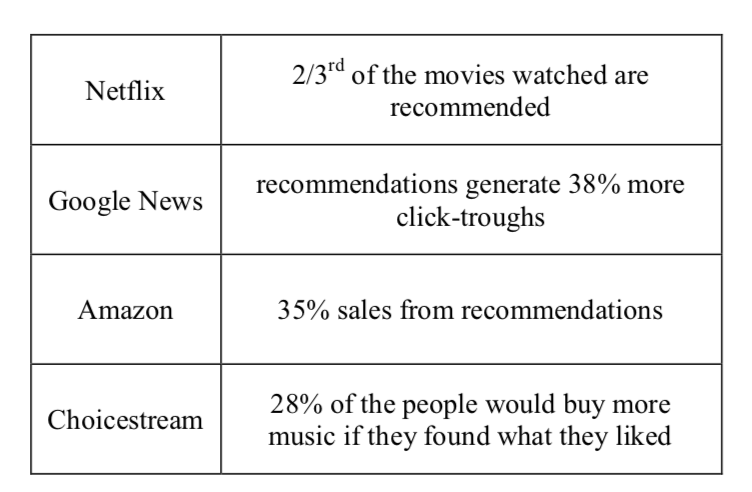
\includegraphics[width=\linewidth]{Figures/successo.png}
        \caption{Successo dei sistemi di raccomandazione di alcune piattaforme \cite{ref1}}
        \label{fig:successo}
    \end{centering}
\end{figure}

Le raccomandazioni fornite dai sistemi di raccomandazioni possono essere accettate oppure ignorate da parte dell'utente. Le interazioni, dirette o indirette, che l'utente ha nei confronti di quanto consigliato dal sistemi formano un insieme di informazioni che sono utilizzate dallo stesso sistema di raccomandazione per migliorare la sua qualità in futuro.

Questi sistemi possono sfruttare modelli, quali il collaborative filtering in modo da incrociare le informazioni di altri utenti ritenuti simili, secondo qualche metrica, per assegnare una valutazione ad un bene non ancora acquistato dall'utente.

Una delle principali sfide dei sistemi di raccomandazione è fornire delle raccomandazioni per gruppi di utenti, bilanciando bisogni e scelte differenti dei vari membri. Un esempio è proprio la raccomandazione di un film ad un gruppo di persone: in questo contesto è possibile riconoscere alcune difficoltà non presenti nel contesto individuale. Alcuni membri del gruppo potrebbero avere interessi competitivi e sarà l'intero gruppo ad accettare o rifiutare la proposta generata.

\section{Collaborative Filtering}

\section{La regola di voto Baewatch}


\begin{table}[]
\centering
\begin{tabular}{|c|c|}
\hline
\multicolumn{1}{|l|}{\textbf{User}} & \multicolumn{1}{l|}{\textbf{Item1}} \\ \hline
User1                               & 4                                   \\ \hline
User2                               & 3                                   \\ \hline
User3                               & 5                                   \\ \hline
User4                               & 2                                   \\ \hline
\end{tabular}
\caption{Successo dei sistemi di raccomandazione di alcune piattaforme \cite{ref1}}
\label{table:1}
\end{table}
        

\section{Esempi di applicazione di Baewatch}
Per concludere la trattazione della regola di voto Baewatch è interessante studiarne l'applicazione su alcuni casi di interesse.

\begin{table}[]
\centering
\begin{tabular}{|l|c|l|}
\hline
\textbf{User}          & \multicolumn{1}{l|}{\textbf{Item1}} & \textbf{Item2} \\ \hline
User1                  & 5                                   & 5              \\ \hline
User2                  & 5                                   & 5              \\ \hline
User3                  & 5                                   & 5              \\ \hline
User4                  & 1                                   & 2              \\ \hline
\textit{Baewatch cost} & \multicolumn{1}{l|}{\textit{16}}    & \textit{9}     \\ \hline
\end{tabular}
\caption{Applicazione di Baewatch ad rating differenti solo per un voto}
\label{table:2}
\end{table}
Nella Tabella \ref{table:2} sono riportati i voti dati da alcuni utenti a due oggetti, \emph{item1} e \emph{item2}. Queste due tuple di voti differiscono solamente per il rating assegnato dall'utente \emph{User4} ai due oggetti: nel primo caso ha attribuito il voto 1 mentre nel secondo il voto 2. Il cambiamento del valore \emph{Baewatch cost} è quindi imputabile solamente a utente \emph{User4} e questo modifica la scelta finale dell'algoritmo dalla prima tupla alla seconda. L'algoritmo preferisce dunque la seconda tupla in quanto presenta un costo inferiore, in linea con il principio di scegliere la tupla "più distante" dal rating minimo.


% \begin{table}[]
% \begin{tabular}{|l|c|l|l|}
% \hline
% \textbf{User}          & \multicolumn{1}{l|}{\textbf{Item1}} & \textbf{Item2} & \textbf{Item3} \\ \hline
% User1                  & 5                                   & 5              & 4              \\ \hline
% User2                  & 5                                   & 5              & 4              \\ \hline
% User3                  & 5                                   & 5              & 4              \\ \hline
% User4                  & 1                                   & 2              & 5              \\ \hline
% \textit{Baewatch cost} & \multicolumn{1}{l|}{\textit{16}}    & \textit{9}     & \textit{3}     \\ \hline
% \end{tabular}
% \end{table}





\begin{table}[]
\centering
\begin{tabular}{|l|l|l|l|l|}
\hline
\textbf{User}          & \textbf{Item1}         & \textbf{Item2} & \textbf{Item3} & \textbf{Item4} \\ \hline
User1                  & \multicolumn{1}{c|}{5} & 5              & 4              & 1              \\ \hline
User2                  & \multicolumn{1}{c|}{5} & 5              & 4              & 1              \\ \hline
User3                  & \multicolumn{1}{c|}{5} & 5              & 4              & 1              \\ \hline
User4                  & \multicolumn{1}{c|}{1} & 2              & 5              & 1              \\ \hline
\textit{Baewatch cost} & \textit{16}            & \textit{9}     & \textit{3}     & \textit{64}    \\ \hline
\textit{Mean}          & \textit{4}             & \textit{4,25}  & \textit{5,25}  & \textit{1}     \\ \hline
\textit{Var}           & \textit{3}             & \textit{2,31}  & \textit{0,15}  & \textit{0}     \\ \hline
\end{tabular}
\caption{Confronto del \textit{Baewatch cost} con \textit{media} e \textit{varianza}}
\label{table:4}
\end{table}

\`E naturale a questo punto proporre un confronto tra la metrica di costo proposta, alla base della regola di voto Baewatch, con media e varianza delle tuple. In Tabella \ref{table:4} sono riportati dei rating di quattro utenti (eventualmente ottenuti attraverso il primo stadio di collaborative filtering) assegnati a due oggetti. Nella tabella sono riportati anche Baewatch cost, media e varianza delle tuple. La quarta tupla è quella che possiede il rating peggiore, tutti gli utenti hanno assegnato il valore minimo; d'altra parte però anche la varianza è minore, indicando che i membri del gruppo sono concordi nella votazione. La varianza effettivamente può essere intesa come una "misura" di quanto i membri del gruppo sono concordi nella votazione. Baewatch ha però come obiettivo massimizzare la "contentezza" del gruppo e non il loro grado di "concordanza". Analizzando sotto questa luce è possibile comprendere allora il perchè del costo maggiore assegnato all quarta tupla: è quella peggiore ottenibile con i voti di quattro utenti espressi nell'intervallo 1-5 e qualsiasi altra tupla sarà sicuramente migliore. La quarta tupla rappresenta effettivamente il punto da cui Baewatch cerca di "allontanarsi".


\begin{table}[]
\centering
\begin{tabular}{|l|c|l|}
\hline
\textbf{User}          & \multicolumn{1}{l|}{\textbf{Item1}} & \textbf{Item2}                   \\ \hline
User1                  & 4                                   & 5                                \\ \hline
User2                  & 4                                   & 5                                \\ \hline
User3                  & 4                                   & 5                                \\ \hline
User4                  & 2                                   & 1                                \\ \hline
\textit{Baewatch cost} & \textit{12}                         & \multicolumn{1}{c|}{\textit{16}} \\ \hline
\textit{Mean}          & \textit{3,5}                        & \multicolumn{1}{c|}{\textit{4}}  \\ \hline
\textit{Var}           & \textit{0,75}                       & \multicolumn{1}{c|}{\textit{3}}  \\ \hline
\end{tabular}
\caption{Baewatch massimizza la "contentezza" del gruppo e non dei singoli componenti}
\label{table:5}
\end{table}

L'ultimo esempio proposto, riportato in Tabella \ref{table:5} è anche quello probabilmente più interessante. \`E possibile infatti notare come la regola di voto assegni un costo minore alla prima tupla anche se la seconda ha media superiore. La Questo fatto è spiegabile considerando che l'idea della regola \emph{Baewatch} è quella di aumentare il grado di "contentezza" dell'\emph{intero} gruppo e non quello dei singoli componenti. L'algoritmo è quindi "disposto" a penalizzare leggermente i primi tre utenti, che comunque mantengono un rating di 4 su 5, per aumentare di uno il voto del quarto membro. Questo comportamento rispecchia quello che avrebbero gruppi di persone nella vita reale: la scelta spesso ricade su una soluzione non ottima, ma comunque non molto lontana da essa, per alcuni componenti per favorire quei pochi membri che in caso contrario otterrebbero la soluzione per loro peggiore.

\section{Conclusioni}


\section{Materiale aggiuntivo}
Una prima implementazione in Pyhton dell'algoritmo presentato è disponibile presso https://github.com/alessandro1105/baewatch. All'interno del repository è possibile trovare il file \emph{test\_complete.py} che permette di valutare l'algoritmo utilizzando il MovieLens 100K Dataset (https://grouplens.org/datasets/movielens/100k/). Il file \emph{test\_paper.py} contiene i test cases presentati in questo documento, insieme ad altri non citati, per dimostrare l'efficacia della regola di voto.

\bigskip
\noindent Thank you for reading these instructions carefully. We look forward to receiving your electronic files!

\bibliographystyle{aaai} 
\bibliography{bibliography}

\end{document}